\section{\name design}

\name uses two techniques, {\em search space pruning} and 
{\em cross-camera profiling}, to reduce the exploration cost.

\subsection{Search space pruning}
The idea behind search space pruning is that the resource-accuracy 
tradeoffs of a configuration tend to be persistent on coarse
timescales, and because of such temporal correlations, we can prune
the space of configurations by avoiding reprofiling those 
configurations that have shown far-from-optimal performance in the 
near past.

%\mypara{Temporal correlation}
To show that the resource-accuracy tradeoffs have {\em temporal 
correlations}, we first examine the timescales on which the 
resource-accuracy tradeoffs of a configuration change. 
Figure~\ref{??} \jc{shows some results}
Besides a substantial temporal correlation, Figure~\ref{??} also
reveals that at any moment, most configurations are far-from-optimal
and remain so for a sustained period of time.

These observations inspire that we should prune the search space of 
configurations, avoiding trying all decisions at the same time.
In particular, \name uses the following algorithm to prune


\subsection{Cross-camera inference}

\begin{figure}[h!]
\centering
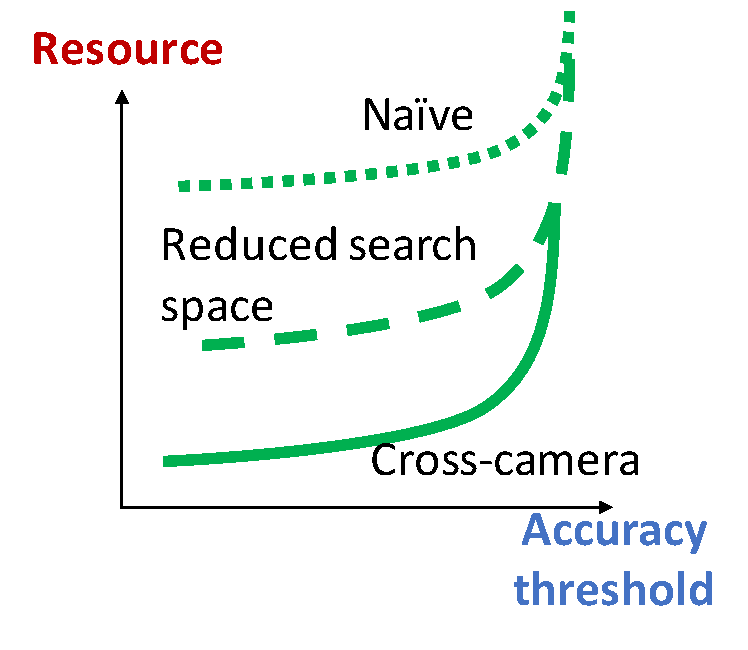
\includegraphics[width=0.35\textwidth]{figures/ReducingCost.pdf}
\vspace{-0.2cm}
\tightcaption{Progressive improvement of search space pruning and 
cross-camera inference.}
\label{fig:}
\end{figure}
